%%%%%%%%%%%%%%%%%%%%%%%%%%%%%%%%%%%%%%%%%%%%%%%%%%%%%%%%%%%%
%  Local Income Taxes and Residential Sorting --- Slide Deck
%  Built on the UMN Gopher Maroon & Gold Beamer template
%%%%%%%%%%%%%%%%%%%%%%%%%%%%%%%%%%%%%%%%%%%%%%%%%%%%%%%%%%%%

\documentclass[xcolor = x11names, compress, aspectratio = 169]{beamer}
\setbeamercovered{transparent}

%%%%%%%%%%%%%%%%  Dependencies %%%%%%%%%%%%%%%%%%%%%%%
\usepackage{graphicx}
\usepackage{booktabs}
\usepackage{textgreek}
\usepackage[round]{natbib}
\usepackage{colortbl}
\usepackage{amsmath}
\usepackage{multirow}
\usepackage{hyperref}

\usefonttheme[onlymath]{serif}
\beamertemplatenavigationsymbolsempty

%% UMN brand colors
\xdefinecolor{GopherMaroon}{HTML}{7A0019}
\xdefinecolor{GopherGold}{HTML}{FFCC33}
\xdefinecolor{GopherLightGold}{HTML}{FFDE7A}
\xdefinecolor{GopherDarkMaroon}{HTML}{5B0013}
%% Utility colors
\definecolor{ForestGreen}{RGB}{34,139,34}
\definecolor{DarkGray}{RGB}{100,100,100}

%%%%%%%%%%%%%%%% Beamer Layout %%%%%%%%%%%%%%%%%%%%%%
\useoutertheme[subsection = false, shadow]{miniframes}
\useinnertheme{default}
\usefonttheme{structureitalicserif}
\usepackage{palatino}
\setbeamerfont{title like}{shape = \scshape}
\setbeamerfont{frametitle}{shape = \scshape}

\setbeamercolor*{lower separation line head}{bg = GopherMaroon}
\setbeamercolor*{normal text}{fg = black, bg = white}
\setbeamercolor*{alerted text}{fg = GopherDarkMaroon}
\setbeamercolor*{example text}{fg = black}
\setbeamercolor*{structure}{fg = GopherDarkMaroon}

\setbeamercolor*{palette tertiary}{fg = GopherMaroon, bg = black!10}
\setbeamercolor*{palette quaternary}{fg = black, bg = black!10}

%% Column shorthand
\renewcommand{\(}{\begin{columns}}
\renewcommand{\)}{\end{columns}}
\newcommand{\<}[1]{\begin{column}{#1}}
\renewcommand{\>}{\end{column}}

%% Footer
\setbeamertemplate{footline}
{
    \leavevmode
    \hbox{%
        \begin{beamercolorbox}[wd = .333333\paperwidth, ht = 2.25ex, dp = 1ex, center]{Author Footer}
            Hockert
        \end{beamercolorbox}
        \begin{beamercolorbox}[wd = .333333\paperwidth, ht = 2.25ex, dp = 1ex, center]{Title Footer}
            Local Income Taxes and Residential Sorting
        \end{beamercolorbox}
        \begin{beamercolorbox}[wd = .333333\paperwidth, ht = 2.25ex, dp = 1ex, right]{Date Footer}
            \usebeamerfont{Date Footer}\today \hspace*{2em}
            \insertframenumber{} / \inserttotalframenumber\hspace*{2ex}
        \end{beamercolorbox}}
        \vskip0pt
    }

\hypersetup{
    colorlinks,
    citecolor = GopherMaroon,
    linkcolor = black
}

\graphicspath{{../figures/}}

%%%%%%%%%%%%%%%%%%%%%%%%%%%%%%%%%%%%%%%%%%%%%%%%%%%%%%%%%%%%%%%%%%%%%%%%
\begin{document}

%%%%%%%%%%%%%%%%%%%%%%%%%%%%%%%%%%%%%%%%%%%%%%%%%%%%%%
%                Title Frame
%%%%%%%%%%%%%%%%%%%%%%%%%%%%%%%%%%%%%%%%%%%%%%%%%%%%%%
\begin{frame}
    \fontfamily{cmr}
    \title{Local Income Taxes and Residential Sorting \\
    \large Evidence from LEHD Origin--Destination Data}
    \author[Hockert]{Matthew Hockert$^\dagger$}
    \date{\small{\textit{\today}}}
    \institute[\textit{UMN}]{
        $^\dagger$\textit{Department of Applied Economics, \\
        University of Minnesota}
    }
    \titlepage
\end{frame}

%%%%%%%%%%%%%%%%%%%%%%%%%%%%%%%%%%%%%%%%%%%%%%%%%%%%%%
\section{Introduction}
%%%%%%%%%%%%%%%%%%%%%%%%%%%%%%%%%%%%%%%%%%%%%%%%%%%%%%

\begin{frame}
\fontfamily{cmr}
\frametitle{Motivation}
    \begin{itemize}\setlength{\itemsep}{0.25cm}
        \item Tiebout (1956): households ``vote with their feet'' across
        local jurisdictions offering different tax/service bundles.
        \item Strong evidence at the state level \citep{kleven2020, young2016}
        and for sales tax cross-border shopping \citep{agrawal2015gradient}.
        \item But little causal evidence on local income tax
        sorting within metros --- where moving costs are small
        and boundaries are frequent.
        \item Two data problems: local tax jurisdictions are sub-county
        (IRS/ACS too coarse), and credit systems + enforcement complicate
        effective tax burden.
    \end{itemize}
\end{frame}

\begin{frame}
\fontfamily{cmr}
\frametitle{This Paper}
    \begin{itemize}\setlength{\itemsep}{0.2cm}
        \item Question: Do local income tax rate changes cause
        residential sorting across municipal boundaries?
        \item Setting: Pennsylvania, 2002--2019. Universal Earned
        Income Tax with continuous rate variation across $\sim$2{,}500
        munis $\times$ $\sim$500 school districts.
        \item Data: LEHD LODES origin--destination, linking
        residence tract $\leftrightarrow$ workplace tract annually.
        \item Outcome: \texttt{share\_live\_in}
        = (workers who live and work in city $i$) / (total workers in $i$),
        plus count outcomes (resident workers, total jobs).
        \item Identification: Act 32 of 2008 (effective Jan.\ 1, 2012)
        consolidated collection and made employer withholding
        mandatory --- a clean enforcement break in the middle of the panel.
    \end{itemize}
\end{frame}

\begin{frame}
\fontfamily{cmr}
\frametitle{Institutional Setting (Pennsylvania)}
    \begin{itemize}\setlength{\itemsep}{0.18cm}
        \item Universal EIT under Act 511 (1965); $\sim$2{,}500 munis
        and $\sim$500 school districts each set rates. Typical 0.5\%
        muni + 0.5\% SD. 291 muni increases, 162 decreases in panel.
        \item Each address has a six-digit \textbf{PSD code} = (muni $\times$ SD)
        identifying its taxing jurisdictions for withholding.
        \item Act 32 of 2008 (eff.\ Jan.\ 1, 2012): consolidated
        collection into 69 Tax Collection Districts; mandated employer
        withholding at the higher of home-resident vs.\ work-nonresident
        rate. Before 2012, withholding fragmented and nonresident
        registry incomplete.
        \item \textbf{Three rates per muni}: $\tau^{\text{res,muni}}$ (residents),
        $\tau^{\text{nr,muni}}$ (nonresidents working there),
        $\tau^{\text{SD}}$ (residents only -- SDs do not levy on nonresidents).
    \end{itemize}
\end{frame}

%%%%%%%%%%% How PA tax works -- piecewise %%%%%%%%%%%
\begin{frame}
\fontfamily{cmr}
\frametitle{How the PA EIT works (post-Act 32, ex.\ Philadelphia)}
    \small
    Worker bill = higher of \emph{total home rate} (muni res + SD) and
    \emph{work-location nonres rate}. Split between cities is piecewise:
    \[
        \bigl(\tau^{\text{home}},\ \tau^{\text{work}}\bigr) =
        \begin{cases}
            \bigl(\tau^{\text{res}}_j + \tau^{\text{SD}}_j - \tau^{\text{nr}}_i,\ \tau^{\text{nr}}_i\bigr)
              & \text{if } \tau^{\text{res}}_j + \tau^{\text{SD}}_j > \tau^{\text{nr}}_i \\[2pt]
            \bigl(0,\ \tau^{\text{nr}}_i\bigr)
              & \text{if } \tau^{\text{res}}_j + \tau^{\text{SD}}_j \leq \tau^{\text{nr}}_i
        \end{cases}
    \]
    \begin{itemize}\setlength{\itemsep}{0.1cm}
        \item Work jurisdiction always collects its full nonresident rate.
        \item Home muni + SD share what's left, zero if work rate is higher.
        \item Which rate binds determines the response margin:
        \emph{home-binds} $\Rightarrow$ move home; \emph{work-binds}
        $\Rightarrow$ change job (or absorb).
    \end{itemize}
\end{frame}

%%%%%%%%%%% Worked numeric example %%%%%%%%%%%
\begin{frame}
\fontfamily{cmr}
\frametitle{Worked example: how this maps to the model}
    \small
    Worker 1 lives in city $B$ (muni 1.0\% + SD 0.5\% = total home 1.5\%) and
    works in city $A$ (muni nonres 0.8\%).
    \begin{itemize}\setlength{\itemsep}{0.08cm}
        \item Bill $= \max(1.5\%, 0.8\%) = 1.5\%$. \textbf{Home binds}.
        $B$ + its SD collect $1.5 - 0.8 = 0.7$pp; $A$ collects $0.8$pp.
        \item In our model: this flow $B \to A$ is treated as a
        \textbf{home-binds observation}. Treatment intensity for
        residential margin = $\tau^{\text{home}}_B = 1.5\%$.
        \item If $B$ raises SD by $0.5$pp (total home now $2.0\%$),
        worker 1's bill rises to $2.0\%$ -- response margin is move home.
        \item If $A$ instead raises nonres to $1.7\%$, regime flips:
        bill $= 1.7\%$ at $A$, home gets $0$. \textbf{Work binds}; worker 1
        can only respond by changing job.
    \end{itemize}
    \vspace{0.1cm}
    \footnotesize Implication: Q2/Q3/Q4 (resident sorting) load on
    $\tau^{\text{res,muni}}_B + \tau^{\text{SD}}_B$. Commuter flow models
    (Q4b/Q6) load on $\tau^{\text{nr}}_A$ at the work side.
\end{frame}

%%%%%%%%%%% Philadelphia handling %%%%%%%%%%%
\begin{frame}
\fontfamily{cmr}
\frametitle{Philadelphia: a separate regime}
    \small
    \begin{itemize}\setlength{\itemsep}{0.15cm}
        \item Philadelphia is \textbf{exempt from Act 32}; its Wage Tax
        operates under the Sterling Act (1932), administered by the
        City Department of Revenue.
        \item Philly residents pay Philly's resident rate
        regardless of where they work --- no max rule, no offset.
        \item Philly nonresidents working in Philly pay Philly's
        nonresident rate to Philly; no residual flows back to home muni.
        \item PA residents who work in Philly: Act 32 does not apply;
        employer withholds Philly nonresident rate.
        \item In our analysis: kept in main sample (it's part of PA's
        labor-market geography), \textbf{excluded in robustness checks}
        because its rate dynamics and reporting differ from Act-32 munis.
    \end{itemize}
\end{frame}

\begin{frame}
\fontfamily{cmr}
\frametitle{Preview of Findings}
    \begin{itemize}\setlength{\itemsep}{0.2cm}
        \item Muni rate increases reduce \texttt{share\_live\_in} by
        $-1.3$ share-points per 1 pp rate hike, building over 7--8 years.
        \item Effect is entirely post-Act 32: muni rate effect is
        a precise zero pre-2012, $-1.8$ share-points** post-2012.
        \item Response is asymmetric: increases push out,
        decreases do not bring back.
        \item School district rate has \emph{opposite sign}: SD
        attracts residents (Q5). The home-side decomposition is
        essential -- bundling muni + SD into a "total" rate hides
        both channels.
        \item City-wide relocation, not boundary arbitrage.
        \item Fiscally productive: EIT revenue $+67\%$,
        total tax $+30\%$, population/property values unaffected.
    \end{itemize}
\end{frame}

%%%%%%%%%%%%%%%%%%%%%%%%%%%%%%%%%%%%%%%%%%%%%%%%%%%%%%
\section{Data}
%%%%%%%%%%%%%%%%%%%%%%%%%%%%%%%%%%%%%%%%%%%%%%%%%%%%%%

\begin{frame}
\fontfamily{cmr}
\frametitle{Data Sources}
    \begin{itemize}\setlength{\itemsep}{0.18cm}
        \item LODES v8 (2002--2019, trimmed pre-COVID):
        tract-pair-year OD flows, main + aux files,
        segments SE01/SE03/SA01-03/JT04.
        \item PA rates: scraped DCED MunStats (resident + nonresident
        muni EIT, school district EIT) $\sim$2{,}500 munis/yr;
        name-based COUSUBFP crosswalk (99.6\% match).
        \item Neighbor pairs: all PA muni pairs within 80 km
        centroid distance ($\sim$1M pairs; regional commute shed).
        \item PA fiscal controls: DCED Annual Financial Reports
        (71 cols: EIT rev, police, fire, streets, sewer, parks,
        comm dev, debt, state aid, pop, MV).
        \item Crime: FBI UCR (Kaplan); Permits: Census BPS.
        \item April 1 alignment between rate panel and LODES
        reference date.
    \end{itemize}
\end{frame}

\begin{frame}
\fontfamily{cmr}
\frametitle{Summary Statistics (Pennsylvania, 2002--2019)}
    \centering
    \small
    \begin{tabular}{lrrrr}
        \toprule
        Variable & Mean & Median & SD & Max \\
        \midrule
        share\_live\_in        & 0.149 & 0.127 & 0.097 & 0.700 \\
        Muni resident EIT (\%) & 0.542 & 0.500 & 0.199 & 4.331 \\
        Muni nonres EIT (\%)   & 0.546 & 0.500 & 0.207 & 4.331 \\
        SD EIT (\%)            & 0.523 & 0.500 & 0.221 & 1.000 \\
        Total jobs             & 3{,}624 & 1{,}224 & & \\
        Resident workers       & 674   & 154   & & \\
        \midrule
        Muni $\times$ year     & \multicolumn{4}{l}{27{,}973 (1{,}479 munis)} \\
        \bottomrule
    \end{tabular}
    \vspace{0.3em}
    \footnotesize \textit{Notes:} Sample restricted to munis with $>50$ total jobs.
    Pre-2012 muni nonres rates backfilled from earliest reported post-2012
    value where missing (96\% of munis stable).
\end{frame}

\begin{frame}
\fontfamily{cmr}
\frametitle{Treatment Geography: PA Rate Changes}
    \centering
    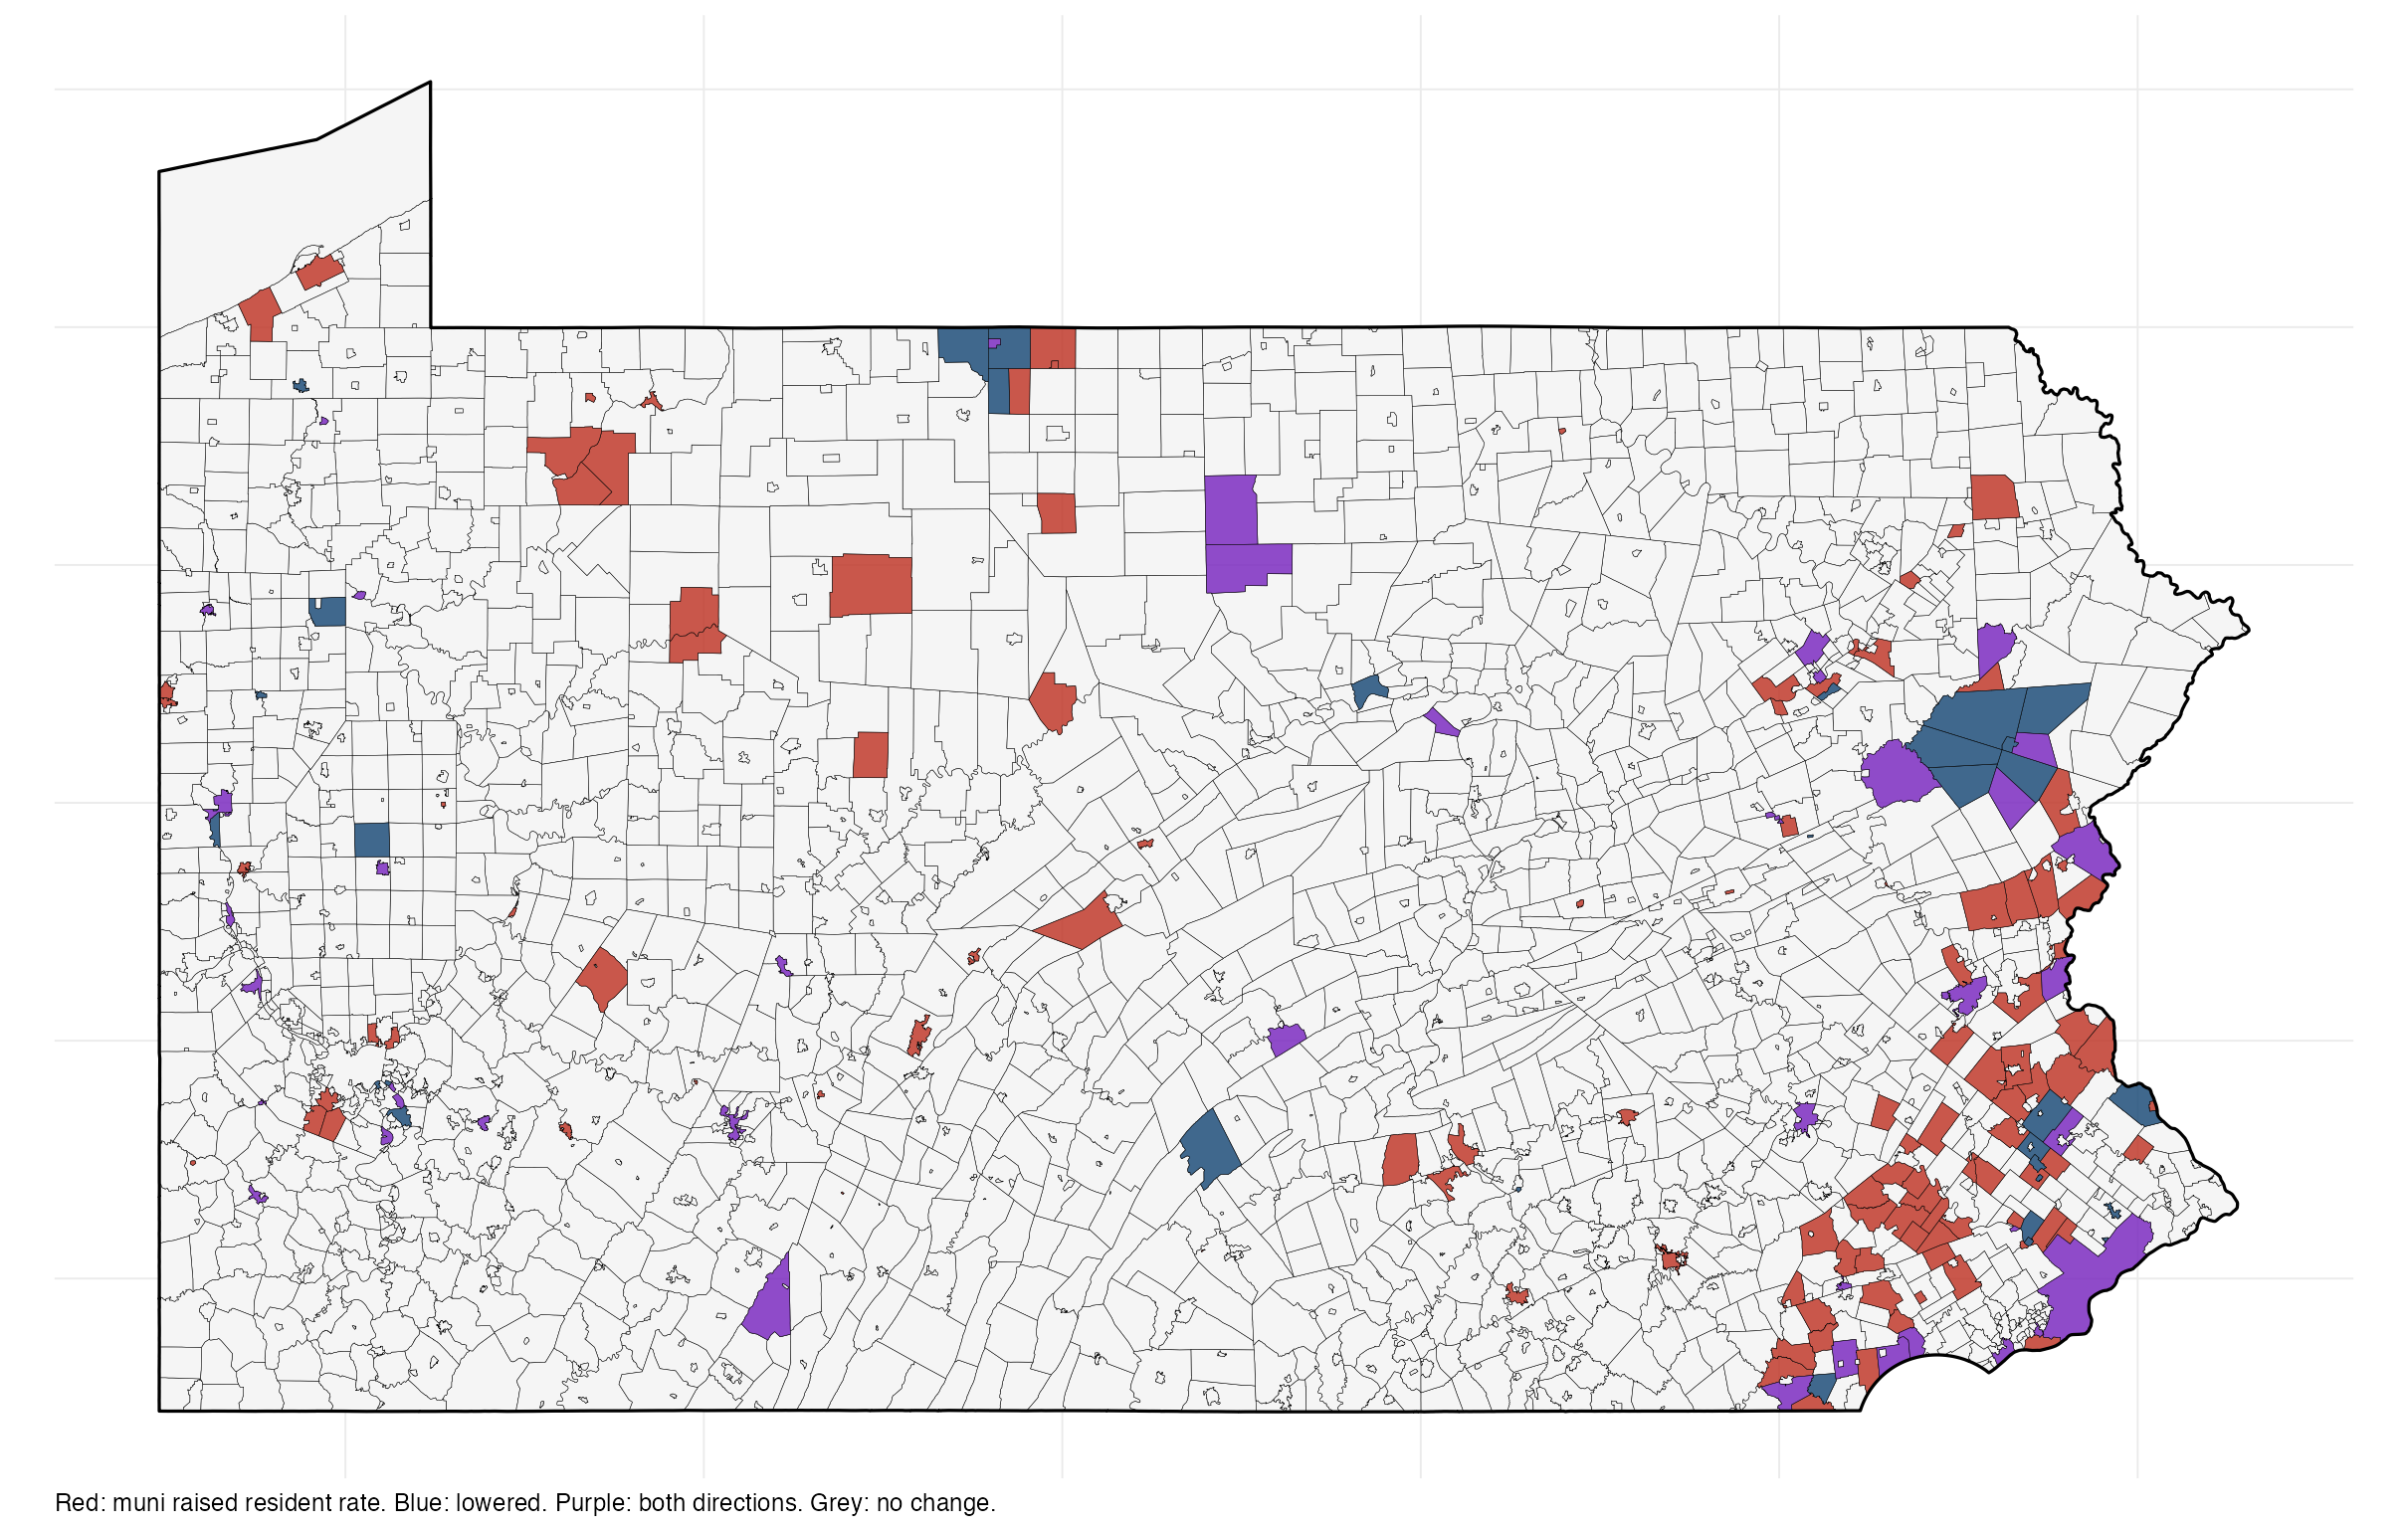
\includegraphics[width=0.72\textwidth]{pa_map.png}
    \vfill
    \small Red = increased; blue = decreased; purple = both; grey = unchanged.
\end{frame}

\begin{frame}
\fontfamily{cmr}
\frametitle{Three Channels of Adjustment}
    When muni $A$ raises its rate, workers in $A$ can:
    \vspace{0.15cm}
    \begin{enumerate}\setlength{\itemsep}{0.15cm}
        \item Move residence only (keep job in $A$).
        Under credit system: liability still $\tau_A$. Zero tax
        savings, but reduces \texttt{share\_live\_in}.
        \item Move residence and job to lower-rate $B$.
        New liability $\tau_B$. Canonical Tiebout margin.
        \item New hires choose to live outside $A$.
        Reduces share even without existing-resident moves.
    \end{enumerate}
    \vspace{0.2cm}
    \footnotesize
    Predictions we'll test:
    (1) enforcement matters $\Rightarrow$ post-Act 32 effect (Act 32 break);
    (2) destination rate irrelevant for commuters when work-binds;
    (3) complete relocators pick lower-rate destinations;
    (4) SD rate opposite sign (Q5);
    (5) boundary gradient (Q6).
\end{frame}

%%%%%%%%%%%%%%%%%%%%%%%%%%%%%%%%%%%%%%%%%%%%%%%%%%%%%%
\section{Methods \& Results}
%%%%%%%%%%%%%%%%%%%%%%%%%%%%%%%%%%%%%%%%%%%%%%%%%%%%%%

%%%%%%%%%%% Q2 (intensive margin -- the headline) %%%%%%%%%%%
\begin{frame}
\fontfamily{cmr}
\frametitle{Q2: Do rate increases cause sorting?}
    \small
    \textbf{Unit $i$ = PA municipality (cousub); $t$ = year, 2002--2019.}
    Outcome \texttt{share\_live\_in}$_{it}$ = workers who live and work
    in muni $i$ at year $t$, divided by total workers in $i$. Workers
    responding pay home stack $\tau^{\text{res,muni}}_i + \tau^{\text{SD}}_i$;
    nonres rate doesn't enter. Three specs:
    \[
    \text{(A) total stack:}\quad Y_{it} = \alpha_i + \gamma_t + \beta\,\tau^{\text{home}}_{it} + \varepsilon_{it}
    \]
    \[
    \text{(B) decomposition:}\quad Y_{it} = \alpha_i + \gamma_t + \beta^{m}\tau^{\text{res,muni}}_{it} + \beta^{sd}\tau^{\text{SD}}_{it} + \varepsilon_{it}
    \]
    \[
    \text{(C) muni only (back-compat):}\quad Y_{it} = \alpha_i + \gamma_t + \beta\,\tau^{\text{res,muni}}_{it} + \varepsilon_{it}
    \]
    \begin{itemize}\setlength{\itemsep}{0.06cm}
        \item Sun--Abraham + DCDH staggered estimators with three cohort
        definitions: muni-rate event, SD-rate event, total-stack event.
        \item Fiscal controls: police, fire, streets, sewer, parks, comm
        dev, gen admin, debt, state aid (full set).
    \end{itemize}
\end{frame}

\begin{frame}
\fontfamily{cmr}
\frametitle{Q2 Answer: muni rate drives the result; SD adds noise}
    \centering
    \small
    \begin{tabular}{lccc}
        \toprule
        & Muni only & Total stack & Decomp \\
        \midrule
        $\tau^{\text{res,muni}}$ & $-0.013^{**}$ & & $-0.013^{**}$ \\
        $\tau^{\text{SD}}$       &               & & $+0.003$ \\
        $\tau^{\text{home}}$     &               & $-0.005$ & \\
        \bottomrule
    \end{tabular}
    \vspace{0.2cm}
    \begin{itemize}\setlength{\itemsep}{0.05cm}\small
        \item Muni rate: $-1.3$ share-pp per 1 pp hike.
        SD rate: zero direct effect on \texttt{share\_live\_in}.
        \item Bundling them dilutes the signal -- SD rate is
        uncorrelated with the sorting margin we measure here.
        \item SD does have effects on resident worker counts (Q5)
        with opposite sign from muni. The decomposition is essential.
    \end{itemize}
\end{frame}

%%%%%%%%%%% Act 32 %%%%%%%%%%%
\begin{frame}
\fontfamily{cmr}
\frametitle{Mechanism: Is it enforcement? (Act 32)}
    \small
    \textbf{Unit $i$ = PA municipality; $t$ = year.} Outcome
    \texttt{share\_live\_in}$_{it}$. Structural break on rate effect:
    \[
    Y_{it} = \alpha_i + \gamma_t
    + \beta^{\text{pre}} \tau_{it} \cdot \mathbf{1}[t<2012]
    + \beta^{\text{post}} \tau_{it} \cdot \mathbf{1}[t\geq 2012]
    + \varepsilon_{it}
    \]
    \begin{itemize}\setlength{\itemsep}{0.08cm}
        \item Pre-2012: fragmented collection, weak withholding;
        DCED's nonresident rate registry was incomplete (only $\sim$55\%
        of munis reported nonres rates; jumped to $\sim$72\% in 2012).
        \item Post-2012: centralized 69 TCDs, mandatory employer
        withholding at $\max(\tau^{\text{home}}, \tau^{\text{nr,work}})$.
        \item Run break for both rates separately to see which channel
        is enforcement-bound.
    \end{itemize}
\end{frame}

\begin{frame}
\fontfamily{cmr}
\frametitle{Act 32 Answer: Sorting only once the tax is binding}
    \centering
    \small
    \begin{tabular}{lcc}
        \toprule
        & Pre-2012 & Post-2012 \\
        \midrule
        $\tau^{\text{res,muni}}$ (muni only)  & $-0.003$ & $-0.018^{***}$ \\
        $\tau^{\text{home}}$ (total stack)    & $-0.005$ & $-0.005$ \\
        $\tau^{\text{res,muni}}$ (decomp)     & $-0.003$ & $-0.017^{***}$ \\
        $\tau^{\text{SD}}$ (decomp)           & $-0.001$ & $+0.007$ \\
        \bottomrule
    \end{tabular}
    \vspace{0.15cm}
    \begin{itemize}\setlength{\itemsep}{0.05cm}\small
        \item Muni rate: precise zero before, $-1.8$ share-pp after.
        Difference significant at 1\%. Same statutory rate, very
        different behavioral response.
        \item Total stack hides the break: SD rate did not get an
        Act-32 enforcement shock (state-administered withholding existed
        already).
        \item Decomposition: enforcement break is on the
        \textbf{muni channel only}. SD plays a different role (Q5).
    \end{itemize}
\end{frame}

%%%%%%%%%%% Q3 %%%%%%%%%%%
\begin{frame}
\fontfamily{cmr}
\frametitle{Q3: Are rate changes symmetric?}
    \small
    \textbf{Unit $i$ = PA municipality; $t$ = year.} Outcome
    \texttt{share\_live\_in}$_{it}$. Split cumulative dose from
    each muni's baseline (first observed) rate:
    \[
    Y_{it} = \alpha_i + \gamma_t + \beta^{+} R^{+}_{it} + \beta^{-} R^{-}_{it} + \mathbf{X}'_{it}\boldsymbol{\phi} + \varepsilon_{it}
    \]
    \begin{itemize}\setlength{\itemsep}{0.08cm}
        \item $R^{+}_{it}$, $R^{-}_{it}$: cumulative increases / decreases from baseline.
        \item If $|\beta^{+}| > |\beta^{-}|$ $\Rightarrow$ residential
        choices are sticky (fixed costs of moving).
        \item Also estimate joint inc/dec event indicators.
    \end{itemize}
\end{frame}

\begin{frame}
\fontfamily{cmr}
\frametitle{Q3 Answer: Sharply asymmetric on muni rate}
    \centering
    \small
    \begin{tabular}{lcc}
        \toprule
        & $R^{+}$ (cum.\ inc) & $R^{-}$ (cum.\ dec) \\
        \midrule
        Muni only & $-0.018^{**}$ & $+0.002$ \\
        Total stack & $-0.006$ & $-0.001$ \\
        Decomp: muni & $-0.018^{***}$ & $+0.001$ \\
        Decomp: SD & $+0.003$ & $+0.019$ \\
        \bottomrule
    \end{tabular}
    \vspace{0.2cm}
    \begin{itemize}\setlength{\itemsep}{0.05cm}\small
        \item Asymmetry on \textbf{muni rate only}: increases push out
        ($-1.8$ share-pp per pp), decreases do not bring back.
        \item SD rate: no asymmetry on share\_live\_in (SD effect lives
        on count outcomes -- Q5).
        \item Policy: a city that raises then lowers its muni rate will
        not recover the residents it lost.
    \end{itemize}
\end{frame}

%%%%%%%%%%% Q4: Where do displaced residents go? %%%%%%%%%%%
\begin{frame}
\fontfamily{cmr}
\frametitle{Q4: Where do displaced residents go?}
    \small
    Two units, two specs:
    \begin{itemize}\setlength{\itemsep}{0.08cm}
        \item \textbf{(a) Resident workers}: unit $B$ = PA municipality;
        $t$ = year. Outcome = log(workers living in $B$, any workplace).
        Full panel; home channel only.
        \[
        \ln(\text{ResW}_{Bt}) = \alpha_B + \gamma_t + \beta_1 \tau^{\text{home}}_{Bt} + \beta_2 \bar{\tau}^{\text{nbr}}_{Bt} + \varepsilon
        \]
        \item \textbf{(b) Commuter flow}: unit = ordered muni-pair $(A,B)$
        with $A \neq B$, within 80 km; $t$ = year. Outcome = log(workers
        commuting from home $B$ to work $A$). Post-Act-32 only.
        \[
        \ln(\text{Flow}_{ABt}) = \alpha_{AB} + \gamma_t + \beta_W \tau^{\text{nr}}_{At} + \beta_H \tau^{\text{home}}_{Bt} + \varepsilon
        \]
    \end{itemize}
    \footnotesize Predictions: $\beta_2 > 0$ in (a) -- neighbors absorb
    displaced residents; $\beta_H \approx 0$ in (b) when work binds
    (credit system makes home rate moot for commuters).
\end{frame}

\begin{frame}
\fontfamily{cmr}
\frametitle{Q4 Answer: Residents leave; neighbors absorb}
    \centering
    \small
    \begin{tabular}{lcc}
        \toprule
        & log(Resident Workers) & Commuter flow $B\to A$ \\
        & home stack on $B$, full panel & post-2012, piecewise \\
        \midrule
        Own muni $\tau^{\text{res,muni}}_B$  & $-0.122^{**}$ & $+0.054^{***}$ \\
        Own SD $\tau^{\text{SD}}_B$           & $+0.147^{***}$ & $\approx 0$ \\
        Neighbor avg                          & $+1.06^{*}$    & --- \\
        Work nonres $\tau^{\text{nr}}_A$      & ---            & $+0.019$ (n.s.) \\
        \bottomrule
    \end{tabular}
    \vspace{0.15cm}
    \begin{itemize}\setlength{\itemsep}{0.05cm}\small
        \item Resident workers in $B$: muni rate repels ($-12\%$ per pp);
        SD rate attracts ($+15\%$). \emph{Neighbors absorb} the displaced
        ($\beta=+1.06^{*}$).
        \item Neighbor = within 80 km centroid distance (regional commute shed).
        \item Commuter flow $B\to A$: work nonres rate near zero (small,
        n.s.). Home muni rate positive on flow -- a \emph{selection
        signature}, not causal: high-rate home cities house residents
        with stronger commuting margins.
        \item Both panels much stronger post-Act-32 (resident-workers
        muni effect $5\times$ larger).
    \end{itemize}
\end{frame}

%%%%%%%%%%% Q5: Muni vs SD decomposition across outcome family %%%%%%%%%%%
\begin{frame}
\fontfamily{cmr}
\frametitle{Q5: Muni vs SD --- decomposition across outcomes}
    \small
    \textbf{Unit $i$ = PA municipality; $t$ = year.}
    Decomposition $\beta^m \tau^{\text{res,muni}}_{it} + \beta^{sd} \tau^{\text{SD}}_{it}$
    estimated for each of four outcomes. Q4 looked at one outcome
    (resident worker count) with neighbor exposure; Q5 fixes the
    decomposition spec and varies the outcome to identify which
    workers respond to which rate.
    \begin{itemize}\setlength{\itemsep}{0.06cm}
        \item Outcomes: \texttt{share\_live\_in}, log(resident workers),
        log(nonresident workers), log(total jobs).
        \item Theory: SD only taxes residents $\Rightarrow$
        $\beta^{sd} \approx 0$ on nonresident outcome but nonzero on
        resident outcomes. Muni res rate same direction across all but
        smaller for nonres workers (who pay only $\tau^{\text{nr,muni}}$,
        which is correlated but not identical).
        \item Muni--SD rate correlation $r=-0.12$ $\Rightarrow$
        independent variation.
    \end{itemize}
\end{frame}

\begin{frame}
\fontfamily{cmr}
\frametitle{Q5 Answer: Opposite signs --- SD attracts residents}
    \centering
    \small
    \begin{tabular}{lcccc}
        \toprule
        & share\_live\_in & log(Resident) & log(Nonres.) & log(Total) \\
        \midrule
        $\tau^{\text{res,muni}}$ & $-0.010^{**}$ & $-0.117^{**}$ & $-0.078^{*}$ & $-0.094^{**}$ \\
        $\tau^{\text{SD}}$       & $+0.002$     & $+0.141^{***}$ & $+0.077$ & $+0.076$ \\
        \midrule
        Total stack & \multicolumn{4}{c}{$\sim 0$ on all -- hides both channels} \\
        \bottomrule
    \end{tabular}
    \vspace{0.15cm}
    \begin{itemize}\setlength{\itemsep}{0.05cm}\small
        \item Muni rate consistently negative; SD strongly positive on
        residents, $\sim 0$ on nonresidents (theory: SDs don't tax commuters).
        \item Bundling them as ``total EIT'' nets to zero $\Rightarrow$
        prior literature using a single rate would find a null.
        \item Decomposition is the methodological contribution.
    \end{itemize}
\end{frame}

\iffalse % HIDDEN: Q6 boundary, Q7 fiscal -- restore by removing iffalse/fi
%%%%%%%%%%% Q6 %%%%%%%%%%%
\begin{frame}
\fontfamily{cmr}
\frametitle{Q6: Is sorting concentrated at municipal boundaries?}
    \small
    Tract-level within-city model. Tract $j$ sits in muni $i$; the
    relevant rate for residents at $j$ is the home stack of $i$.
    \[
    S^{\text{within}}_{jt} = \alpha_j + \gamma_t + \beta_1 \tau^{\text{home}}_{it} + \beta_2 \tau^{\text{home}}_{it} \times \mathbf{1}[\text{boundary}_j] + \varepsilon_{jt}
    \]
    \begin{itemize}\setlength{\itemsep}{0.08cm}
        \item $S^{\text{within}}_{jt}$ = share of workers at tract $j$
        whose home is also in $i$. Boundary tract = centroid within 1 km
        of nearest muni boundary.
        \item Prediction 5: $\beta_2<0$ if cross-boundary tax arbitrage
        dominates (boundary tracts lose residents to neighbors).
        \item Total-workers (denominator) spec adds work nonres rate
        and is post-Act-32 only.
        \item Also estimate distance-to-boundary gradient
        (0--0.5, 0.5--1, 1--2, 2--5, 5+ km).
    \end{itemize}
\end{frame}

\begin{frame}
\fontfamily{cmr}
\frametitle{Q6 Answer: No boundary gradient --- city-wide response}
    \centering
    \small
    \begin{tabular}{lcc}
        \toprule
        & Within-city share & log(Total workers) \\
        \midrule
        Muni EIT             & $+0.0006^{**}$ $(0.0003)$ & $+0.0217^{***}$ $(0.0027)$ \\
        Muni EIT $\times$ Boundary & $+0.0008$ $(0.0013)$  & $-0.0449^{*}$ $(0.0266)$ \\
        \bottomrule
    \end{tabular}
    \vspace{0.2cm}
    \begin{itemize}\setlength{\itemsep}{0.05cm}
        \item Within-city reshuffling: essentially zero $\Rightarrow$
        people are crossing muni boundaries, not just neighborhoods.
        \item Boundary $\times$ rate on share: null. Boundary tracts
        respond like interior tracts.
        \item Boundary tracts do lose total workers marginally ($-4.5\%^{*}$),
        hinting at employment leaking across boundaries.
        \item Consistent with whole-city relocation, not short-distance tax arbitrage.
    \end{itemize}
\end{frame}

%%%%%%%%%%% Q7 %%%%%%%%%%%
\begin{frame}
\fontfamily{cmr}
\frametitle{Q7: Where does the incremental revenue go?}
    \small
    Expenditure decomposition (AFR):
    \[
    \ln(\text{Exp}^{k}_{it}) = \alpha_i + \gamma_t + \beta^{k} \tau_{it} + \varepsilon_{it}
    \]
    $k \in \{$police, fire, streets, admin, debt, sewer, rec, comm dev$\}$.
    \vspace{0.1cm}

    Does visibility of spending moderate sorting?
    \[
    Y_{it} = \alpha_i + \gamma_t + \beta_1 \tau_{it} + \beta_2 \tau_{it} \times S^{\text{visible}}_i + \varepsilon_{it}
    \]
    $S^{\text{visible}}_i$ = pre-treatment share on police + fire + streets.
\end{frame}

\begin{frame}
\fontfamily{cmr}
\frametitle{Q7 Answer: Revenue funds invisible community dev}
    \centering
    \small
    \begin{tabular}{lccccc}
        \toprule
        & EIT Rev & Police & Fire & Streets & Comm Dev \\
        \midrule
        $\tau^{\text{res,muni}}$ & $+0.67^{***}$ & $+0.05$ & $+0.09^{*}$ & $+0.09^{**}$ & $+0.92^{***}$ \\
        $\tau^{\text{SD}}$       & $-0.06^{***}$ & $-0.10$ & $+0.16^{***}$ & $+0.08^{**}$ & $+0.05$ \\
        \bottomrule
    \end{tabular}
    \vspace{0.2cm}
    \begin{itemize}\setlength{\itemsep}{0.05cm}\small
        \item Muni rate funds long-horizon community development
        ($+92\%^{***}$); police unmoved.
        \item SD rate funds fire and streets at the muni level (cross-budget
        substitution effect); negative on EIT revenue is an institutional
        artifact (PA AFR reports muni-only revenue, SD has separate accounts).
        \item Interpretation: rate increases fund hard-to-see investments.
        Residents don't see more patrols, which limits visibility-driven
        offset to the sorting cost.
    \end{itemize}
\end{frame}
\fi % END HIDDEN: Q6 + Q7

%%%%%%%%%%%%%%%%%%%%%%%%%%%%%%%%%%%%%%%%%%%%%%%%%%%%%%
\section{Robustness}
%%%%%%%%%%%%%%%%%%%%%%%%%%%%%%%%%%%%%%%%%%%%%%%%%%%%%%

\iffalse % HIDDEN: Fiscal Impact slide -- restore by removing iffalse/fi
\begin{frame}
\fontfamily{cmr}
\frametitle{Fiscal Impact: Rates ``Work''}
    \centering
    \small
    \begin{tabular}{lcccccc}
        \toprule
        & log(EIT) & log(Tot.\ Tax) & log(Tot.\ Rev) & log(Police) & log(Pop) & log(MV) \\
        \midrule
        $\tau^{\text{res}}$ & $0.671^{***}$ & $0.296^{***}$ & $0.064$ & $0.053$ & $-0.009$ & $0.007$ \\
                             & $(0.211)$ & $(0.095)$ & $(0.043)$ & $(0.046)$ & $(0.014)$ & $(0.022)$ \\
        \bottomrule
    \end{tabular}
    \vspace{0.2cm}
    \begin{itemize}\setlength{\itemsep}{0.05cm}
        \item EIT revenue $+67\%^{***}$, total tax $+30\%^{***}$ per 1 pp of rate increase.
        \item Population, property values, total revenue: null.
        \item Behavioral response too small to erode the base
        --- rate increases are on the right side of the revenue hill.
    \end{itemize}
\end{frame}
\fi % END HIDDEN: Fiscal Impact

\begin{frame}
\fontfamily{cmr}
\frametitle{Robustness}
    \begin{itemize}\setlength{\itemsep}{0.15cm}
        \item Pre-trends clean across 11 observables: revenue,
        EIT rev, RE tax, streets, pop, debt, jobs, crime, permits.
        Exceptions (police, market value) addressed with controls /
        coverage notes.
        \item Fiscal controls (log police, streets, debt, state aid)
        leave point estimates and SEs essentially unchanged.
        \item Philadelphia exclusion: results robust to dropping Philly.
        \item Flip-floppers: 37\% of PA treated munis flip-flop;
        excluding them strengthens results.
        \item Placebo: Federal workers (JT04) show no response
        (federal wages not subject to local withholding same way).
        \item ACS / IRS SOI: county-level migration null ---
        LODES detects what coarser data cannot.
    \end{itemize}
\end{frame}

%%%%%%%%%%%%%%%%%%%%%%%%%%%%%%%%%%%%%%%%%%%%%%%%%%%%%%
\section{Conclusion}
%%%%%%%%%%%%%%%%%%%%%%%%%%%%%%%%%%%%%%%%%%%%%%%%%%%%%%

\begin{frame}
\fontfamily{cmr}
\frametitle{Putting it Together (1/2): Who moves?}
    \small
    \textsc{Setup.} A post-Act 32 PA city: 1{,}000 total workers;
    150 live-and-work there (share\_live\_in = 15\%); EIT rises
    0.5\% $\rightarrow$ 1.5\%.
    \vspace{0.2cm}
    \begin{itemize}\setlength{\itemsep}{0.15cm}
        \item[Q2/Q3.] Over 7--8 years, share falls to $\sim$13.2\% $\Rightarrow$
        $\sim$18 of 150 locally-resident workers gone. If the city later
        cuts the rate back, none of them return.
        \item[Q4.] Those 18 leave the city entirely (not a neighborhood move);
        nearby lower-rate munis within 80 km absorb them.
        \item[Q5.] If the overlapping school district had raised its rate
        instead, residents would have moved in, not out.
        \item[Q6.] The loss is spread across the city, not concentrated
        at municipal boundaries --- no ``edge effect.''
    \end{itemize}
\end{frame}

\begin{frame}
\fontfamily{cmr}
\frametitle{Putting it Together (2/2): Was it worth it?}
    \small
    Same city: 1{,}000 workers, rate 0.5\% $\rightarrow$ 1.5\%, $\sim$18 residents lost.
    \vspace{0.2cm}
    \begin{itemize}\setlength{\itemsep}{0.15cm}
        \item[Fiscal.] EIT revenue roughly doubles ($+67$ log points);
        total tax $+30\%$. Property values and population: unchanged.
        \item[Q7.] Most new dollars flow to community development
        (planning, econ dev, housing) --- not to police patrols residents see.
        \item[Enforcement.] None of this happens pre-Act 32: same statutory
        rate, precise zero behavioral response. Collection capacity is the
        binding constraint.
    \end{itemize}
    \vspace{0.3cm}
    \textsc{Bottom line.} The city trades $\sim$18 residents for a near
    doubling of EIT revenue. Rate increases work --- when enforced.
\end{frame}

\begin{frame}
\fontfamily{cmr}
\frametitle{Summary}
    \begin{enumerate}\setlength{\itemsep}{0.15cm}
        \item Local income tax rate increases cause residential sorting:
        \texttt{share\_live\_in} falls by 0.5--0.8 share-points per 1 pp
        rate hike, building over 7--8 years.
        \item Effect is enforcement-contingent: zero pre-Act 32,
        large post-2012.
        \item Sorting is asymmetric (sticky residences) and
        city-wide (not boundary arbitrage).
        \item Muni and SD rates have opposite signs ---
        SD acts as an amenity.
        \item Rate increases are fiscally productive: base erosion
        too small to offset revenue gains.
    \end{enumerate}
\end{frame}

\begin{frame}
\fontfamily{cmr}
\frametitle{Next Steps}
    \begin{itemize}\setlength{\itemsep}{0.15cm}
        \item Link Act 1 SD rate changes to actual property tax millage
        movements (PDE data 2015+ restrictive).
        \item Extend Q7 with richer, pre-treatment expenditure
        composition (more power on visibility channel).
        \item Apply the LODES-based design to other local instruments
        (property tax millage, local sales taxes, fees).
        \item Welfare: combine behavioral elasticity with revenue
        elasticity to bound efficiency cost of local income tax.
    \end{itemize}
\end{frame}

\begin{frame}
\fontfamily{cmr}
\frametitle{Thank You}
    \centering
    \vfill
    \Large Questions?
    \vfill
    \normalsize
    \texttt{hocke043@umn.edu} \\
    \small github.com/MatthewHockert/local-income-tax-migration
    \vfill
\end{frame}

\end{document}
